\documentclass[tikz,border=4pt]{standalone}
\usepackage{amsmath,amssymb}
\usepackage{tikz}
\usetikzlibrary{arrows.meta}

\begin{document}
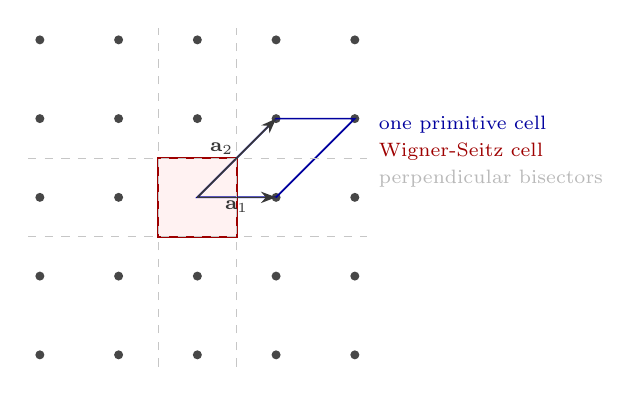
\begin{tikzpicture}[
  >=Stealth,
  point/.style={circle, fill=black!72, inner sep=1.15pt},
  guide/.style={dashed, gray!45, line width=0.28pt},
  cell/.style={line width=0.62pt, blue!62!black},
  ws/.style={line width=0.72pt, red!62!black},
  vec/.style={->, line width=0.55pt, black!78},
  every node/.style={font=\scriptsize}
]
  \foreach \i in {-2,-1,0,1,2} {
    \foreach \j in {-2,-1,0,1,2} {
      \node[point] at (\i,\j) {};
    }
  }

  \fill[red!5] (-0.5,-0.5) rectangle (0.5,0.5);
  \draw[ws] (-0.5,-0.5) rectangle (0.5,0.5);
  \draw[cell] (0,0) -- (1,0) -- (2,1) -- (1,1) -- cycle;

  \draw[guide] (-0.5,-2.15) -- (-0.5,2.15);
  \draw[guide] (0.5,-2.15) -- (0.5,2.15);
  \draw[guide] (-2.15,-0.5) -- (2.15,-0.5);
  \draw[guide] (-2.15,0.5) -- (2.15,0.5);

  \draw[vec] (0,0) -- node[below, inner sep=1pt] {$\mathbf a_1$} (1,0);
  \draw[vec] (0,0) -- node[above left, inner sep=1pt] {$\mathbf a_2$} (1,1);

  \node[blue!62!black, anchor=west] at (2.18,0.92) {one primitive cell};
  \node[red!62!black, anchor=west] at (2.18,0.58) {Wigner-Seitz cell};
  \node[gray!55, anchor=west] at (2.18,0.24) {perpendicular bisectors};
\end{tikzpicture}
\end{document}
